\chapter{Segmentation methods based on Intensity Similarity}
\section{Otsus Segmentation}\index{Otsus Otsus Segmentation}
In computer vision and image processing, \textbf{Otsu's} method, named after \textbf{Nobuyuki Otsu}, is used to automatically perform clustering-based image thresholding, the reduction of a graylevel image to a binary image. The algorithm assumes that the image contains two classes of pixels following bi-modal histogram (foreground pixels and background pixels), it then calculates the optimum threshold separating the two classes so that their combined spread (intra-class variance) is minimal, or equivalently (because the sum of pairwise squared distances is constant), so that their inter-class variance is maximal. Consequently, Otsu's method is roughly a one-dimensional, discrete analog of Fisher's Discriminant Analysis. Otsu's method is also directly related to the Jenks optimization method.
\\
\\
\textbf{Otsu's Algorithm:}
\begin{enumerate}
\item Compute histogram and probabilities of each intensity level
\item Set up initial $w_i(0)$ and $u_i(0)$.
\item Step through all possible thresholds \textit{t=1,....}  maximum intensity.
  \begin{enumerate}
  \item Update $w_i$ and $u_i$.
  \item Compute $\sigma_{b}^{2}$(t)
  \end{enumerate}
\item Desired threshold corresponds to the maximum $\sigma_{b}^{2}$ (t).
\end{enumerate}

Otsu’s method exhibits the relatively good performance if the histogram can be assumed to have bimodal distribution and assumed to possess a deep and sharp valley between two peaks. But if the object area is small compared with the background area, the histogram no longer exhibits bimodality. And if the variances of the object and the background intensities are large compared to the mean difference, or the image is severely corrupted by additive noise, the sharp valley of the gray level histogram is degraded. Then the possibly incorrect threshold determined by Otsu’s method results in the segmentation error. (Here we define the object size to be the ratio of the object area to the entire image area and the mean difference to be the difference of the average intensities of the object and the background).

\section{Inclass Images}\index{Inclass Images working}
\subsection{Image \texttt{10\_27a}}
\begin{figure}[h!]
  \centering
  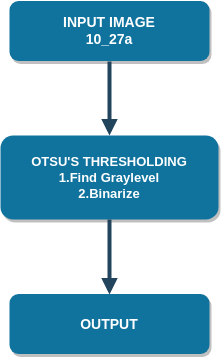
\includegraphics[width=6cm,height=10cm,keepaspectratio]{img/image_10_27a_flow.png}
  \caption{Image \textttt{10\_27a} workflow}
\end{figure}

This image was pretty straight forward and did not require any pre-processing. We used Otsu’s Segmentation to obtain the output image.

\pagebreak

\subsection{Image \texttt{10\_27d}}
\begin{figure}[h!]
  \centering
  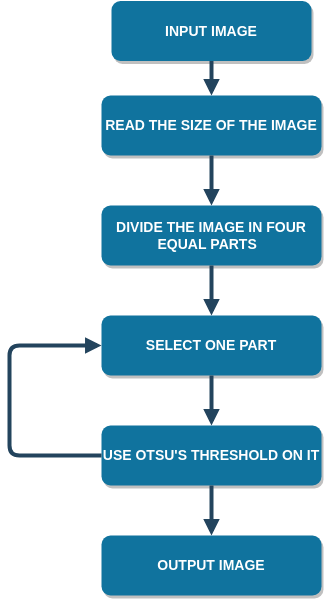
\includegraphics[width=8cm,height=15cm,keepaspectratio]{img/10_27d_flow.png}
  \caption{Image \textttt{10\_27d} workflow}
\end{figure}

The image had non-uniform background as well as foreground and it was positioned in such a way that applying Otsu’s Segmentation would not produce the deserved image. The gray level of one side of the object was same as the gray level of the background on the other side. Thus the gray level threshold obtained from Otsu’s Segmentation would not do justice with the image. It was not able to segment object from the background.
\\
\\
To overcome this problem, we strategize to break the image to four equal halves. The gray level difference in background and foreground of each of these blocks was sufficient enough to use Otsu’s Segmentation on it.
\\
\\
This method gave us a good result with very less error.

\section{Extra Images}\index{Extra Images workings}
\subsection{Image \textttt{group of coins}}
\begin{figure}[h!]
  \centering
  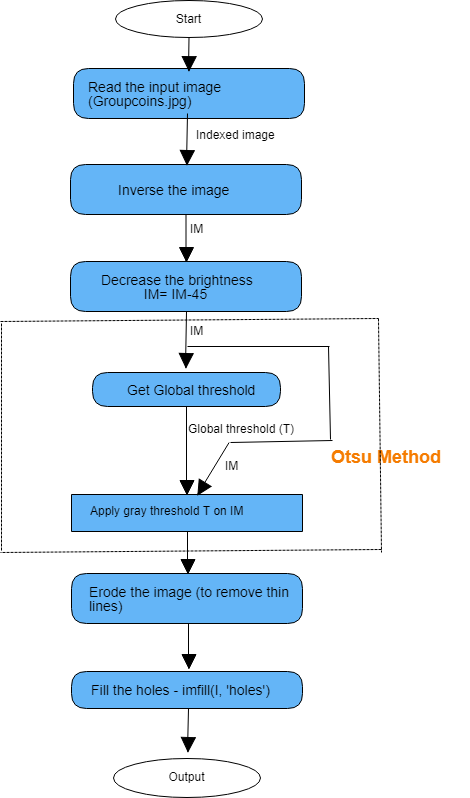
\includegraphics[width=10cm,height=18cm,keepaspectratio]{img/grp_of_coins_flow.png}
  \caption{Image \textttt{grp\_of\_coins} workflow}
\end{figure}

For the image \texttt{group\_of\_coins.png}, our goal was to segment the coins from the background, In the image as the background is white, but we wanted objects in white and background in black, we applied inverse of the image and processed the resultant image with the further steps. As the inversed image is very bright and that might affect the output so we have decreased the brightness of image first and then we used Otsus method for image segmentation and were able to segment the coins from the background, but there was some extra lines on coins, so we eroded the image to remove thin lines and finally we filled the holes if there are any as the coins are closed objects. With Otsus segmentation and eroding the image, we successfully segmented the coins from the background.

\subsection{Image \texttt{jet\_fighter\_swarms}}
This image has the objects in gray color and background is light color so we have first inversed the image as our goal was to have the objects segmented from the background with objects as white in color and background as black color. Then we decreased the brightness as some of the background pixels are bright after inverse. We then applied Otsus thresholding method and achieved the objects segmented successfully.

\section{Adaptive Thresholding}\index{Adaptive Thresholding}
Thresholding is the simplest way to segment objects from a background. If that background is relatively uniform, then you can use a global threshold value to binarize the image by pixel-intensity. If there’s large variation in the background intensity, however, \textbf{adaptive thresholding} (a.k.a. local or dynamic thresholding) may produce better results.
\\
Here, we binarize an image using the threshold adaptive function, which calculates thresholds in regions of size block size surrounding each pixel (i.e. local neighborhoods). Each threshold value is the weighted mean of the local neighborhood minus an offset value.
\\
\\
Adaptive thresholding is useful for segmenting variable background images. It changes the image threshold dynamically, as opposed to applying a monotonous threshold to all the pixels in the image. Each pixel is considered to have a local neighborhood of n x n pixels, the mean or median of which is used to calculate the local threshold value. 
\\
The pixel that we are taking into consideration is set to black or white depending on whether it falls below or above this local threshold value. The technique can be improved by employing an additive constant, which can be subtracted from the calculated mean or median of the \texttt{n x n} neighborhood. The technique is successful at adapting for variations in the background if the \texttt{n x n} neighborhood is of an optimal size.

\subsection{Image \texttt{son1.gif}}
\begin{figure}[h!]
  \centering
  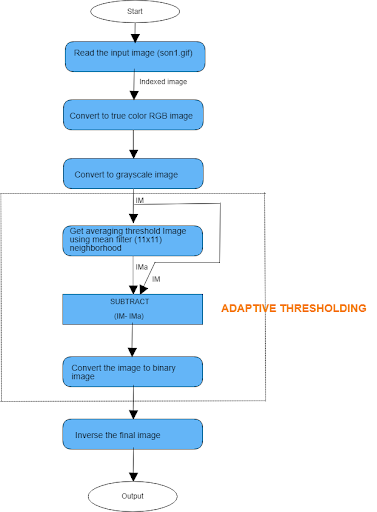
\includegraphics[width=10cm,height=18cm,keepaspectratio]{img/son1_flow.png}
  \caption{Image \textttt{son1} workflow}
\end{figure}

Our Goal is to segment the text from the background from the image son1.gif. But the image son1.gif has a varying background, a single threshold is unsuitable for the entire image field for separating the text from the background. Instead, it is preferable to implement some form of per-pixel thresholding, in which a different threshold is computed for every pixel (i.e. a "threshold image"), so we have choose adaptive thresholding method for this image segmentation.
\\
\\
As we found that, a single threshold (Otsus method) fails segmenting the text for this source image. Instead of using a single number or global threshold, we established the threshold for each pixel by taking mean average of the brightness values in its neighborhood (minus a constant value of \texttt{0.025}). For this image we have taken \texttt{(11x11)} neighborhood pixels to calculate average mean threshold. The average threshold of the image is then subtracted from the input gray level image and final segmented image is achieved. With this method we were able to successfully segment the text from the background.

\pagebreak

\subsection{Image \texttt{papir}}
\begin{figure}[h!]
  \centering
  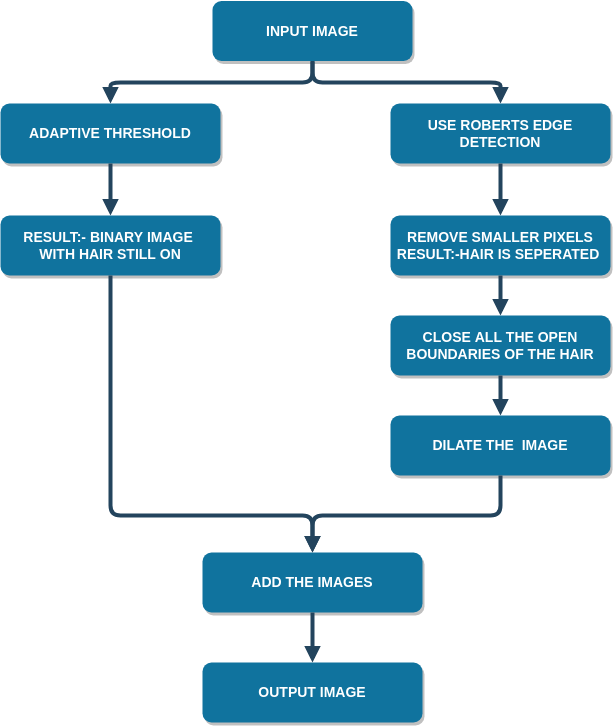
\includegraphics[width=12cm,height=18cm,keepaspectratio]{img/papir_flow.png}
  \caption{Image \textttt{papir} workflow}
\end{figure}
Objective for this image was
\begin{enumerate}
  \item To remove the hair from the image.
  \item To alter the uneven illumination in the background.
\end{enumerate}

We started the process of hair removal using Roberts edge detection. We then removed the the small pixels to isolate the hair in the image. Then we performed bwclose on the result image to close any open boundaries. After which we dilated the image which was basically done to thicken the size of the hair. Now we had image with black background and clear thick hair in white. We solved the uneven illumination problem by using  adaptive thresholding, which produced a binary image with with white background and text, hair in black.
\\
We added both the image producing a binary image without the hair.
%%% Local Variables:
%%% mode: latex
%%% TeX-master: t
%%% End:
